% Draft No. 2
  % Description
  % Instructions
% Practice
  % Example: ESS dataset
  % Practice session

\documentclass[t]{beamer}
\usetheme{\usetheme{hkllite}}

\title{revised draft}
	\author{François Briatte \& Ivaylo Petev}
	\date{Week~\#10}

\begin{document}
	
    \frame[plain]{
		\titlepage\\[7em]
		\tableofcontents[hideallsubsections]
		}

	%
	%

	%
	%
	\section{Draft No. 2}	
	%
	%
	
	%
	%
	\subsection{Description}
	%
	%
	
	\begin{frame}[t]{Draft No.~2}
	
	\begin{columns}[T]
		\column{.3\textwidth}

			\textbf{Univariate\\statistics}\\[.5em]
	
			\begin{itemize}
				\item Introduction
				% (topic)
				\item Datasets
				% (observations and variables)
				\item Distributions
				% (central tendency, variability, normality)
				\item Estimation
				% (PDF, CLT, LLN, CIs)
			\end{itemize}
			
			$$
			\left.
			    \begin{array}{rrr}
			        corrected \\
			        revised\\
			        appended
			    \end{array}
			\right \} 
			$$	
		
		\column{.3\textwidth}
		
			\textbf{Bivariate\\statistics}
	
			\begin{itemize}
				\item Significance
				% (comparison of means and proportions)
				\item Comparisons
				% (t-test, Chi-squared test)
				\item Correlation
				% (scatterplot and correlation matrixes)
				\item Regression
				% (Simple OLS linear regression)
			\end{itemize}
			
			\begin{center}
				\red{Revised draft}\\[.5em]
				\fbox{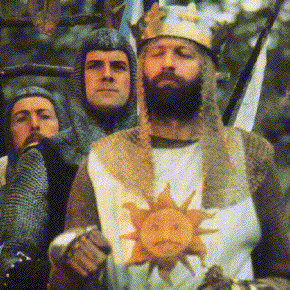
\includegraphics[width=.75\textwidth]{holy-grail2.jpg}}
			\end{center}
		
		\column{.3\textwidth}

			\textbf{Statistical\\modelling}
	
			\begin{itemize}
				\item Basics
				% (residuals)
				\item Extensions
				% (dummies)
				\item Diagnostics
				% (multicollinearity, heteroscedasticity)
				\item Conclusion
				% (extensions)
			\end{itemize}

			\begin{center}
				Final paper\\[.5em]
				\fbox{
\includegraphics[width=.75\textwidth]{holy-grail.jpg}}
			\end{center}
			
	\end{columns}
		
	\end{frame}
	%
	%

	%
	%
	\subsection{Instructions}
	%
	%

	\begin{frame}[t]{First steps}

	\begin{block}{Go through corrections}
	
		\begin{itemize}
			\item Remove technical content
			\item \red{Rewrite until concision}
		\end{itemize}

	\end{block}
	
	\begin{block}{Explore associations}

		\begin{itemize}
			\item Stata Guide, Sec.~10 \hfill%
				\code{ttest}, \code{prtest}, \code{tab,~chi2}, \code{pwcorr}
			\item Stata Guide, Sec.~11 \hfill%
				\code{sc}, \code{lowess}, \code{pwcorr}, \code{reg}, \code{rvfplot}
		\end{itemize}
		
		Write up \red{substantive results} as sentences; %
		cite significance tests and other statistics in brackets: %
		$(\rho = .7)$, $(p < .05)$, …
			
	\end{block}

	\end{frame}
	%
	%

  \begin{frame}[c]{Draft regressions}
  
	\begin{block}{Model choice}
	
		\begin{itemize}
			\item \textbf{Linear model} if the DV is continuous \hfill %
				\code{reg}
				
				$$Y = \beta_0 + \beta_1 X_1 + \beta_2 X_2 + \epsilon$$
				
			\item \textbf{Logistic model} if the DV is discrete \hfill %
				\code{logit}
				
				$$Pr(Y = 1) = \frac{exp(\beta_0 + \beta_1 X_1 + \beta_2 X_2 + \epsilon)}%
				{1 + exp(\beta_0 + \beta_1 X_1 + \beta_2 X_2 + \epsilon)}$$
				
		\end{itemize}

	\end{block}

	\begin{block}{Model operations}

		\begin{itemize}
			\item Estimation and diagnostics
			\item Export and \red{interpretation}
		\end{itemize}
		
	\end{block}
	
  \end{frame}
	%
	%

	%
	%
	\section{Practice}
	%	
	%

	%
	%
	\subsection{Example: ESS dataset}
	%
	%
	
	\begin{frame}[t]{Practice: \red{ESS dataset}}

		\begin{columns}[c]
			\column{.55\textwidth}

	    Data:\\[.5em]

			\begin{itemize}
				\item European Social Survey (ESS)
				\item Sample: individuals, c.~2008
			\end{itemize}
		
			\vspace{.75em}
		
	    Dependent variable:\\[.5em]
		
			\begin{quote}
			  To what extent do you think [country] should allow %
				many/few immigrants of different race/ethnic group %
				from majority?				
			\end{quote}
	
			\column{.35\textwidth}

			
\includegraphics[width=.6\textwidth]{logo-ess}

		\end{columns}
	
	\end{frame}
	%
	%
	
	%
	%
	\subsection{Practice session}
  %
  %
  
	\begin{frame}[t]{Practice session}

    \begin{block}{Class}
      \comm{Get the do-file for this week.}\\
      \code{srqm\_get week10.do}\\
      
			\comm{Open to read and replicate.}\\
			\code{doedit code/week10}\\    
    \end{block}

    \begin{alertblock}{Coursework}
      \begin{itemize}
	      \item Finish the do-file and read all comments at home.
	      \item Add draft regressions to your do-file.
	      \item Add draft regression results to your paper.
      \end{itemize}
    \end{alertblock}
    		
	\end{frame}
  %
  %
	
\end{document}
